%!TeX program=xelatex
\documentclass[a4paper]{article}

\usepackage{amsmath}
\usepackage{amssymb}
\usepackage[margin=1in]{geometry}
\usepackage{xcolor}
\usepackage{hyperref}
\hypersetup{
    colorlinks,
    linkcolor={red!50!black},
    citecolor={blue!50!black},
    urlcolor={green!50!black}
}
\usepackage{subcaption}

\usepackage{fontspec}
\setmainfont{Latin Modern Roman}

\renewcommand{\vec}{\boldsymbol}
\newcommand{\vectilde}[1]{\tilde{\boldsymbol{#1}}}

\begin{document}
    \title{Machine Learning with Crowdsourced Labels on the Radio~Galaxy~Zoo}
    \author{Matthew Alger \\ \emph{The Australian National University}}
    \maketitle

    \section{The Radio Galaxy Zoo}

        In this section, I will introduce the Radio Galaxy Zoo, the problem it aims to solve, and how this relates to my project.

        \emph{Black holes} are masses that are so dense that even light cannot escape their gravitational field. Supermassive black holes are found at the centre of most galaxies, but astronomers don't know a great deal about them or their interactions with the galaxy surrounding them, which is called the \emph{host galaxy}. To find out more, astronomers need to look at many different black holes and their host galaxies. The host galaxies turn out to be particularly important: You can't get a lot of information from looking at a black hole by itself. Even simple things like how big the black hole is need more information, and this information comes from the host galaxy. From this, it's apparent that even if we have observations of black holes, we need to know what galaxy hosts them.

        \begin{figure}[!ht]
            \center
            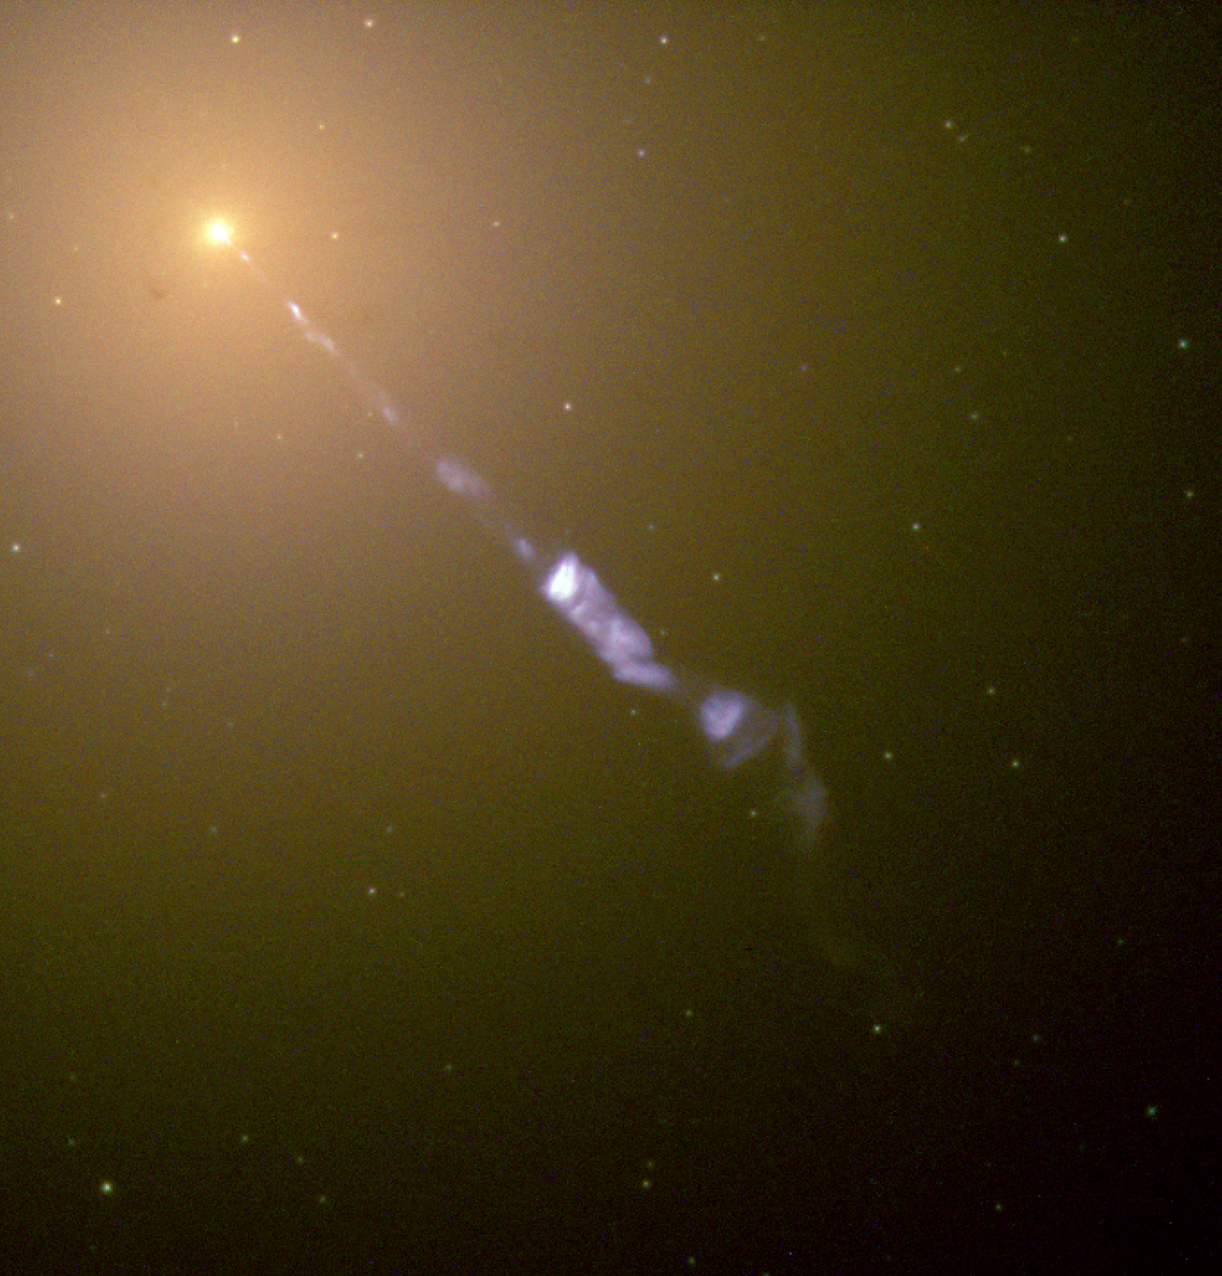
\includegraphics[width=.3\textwidth]{images/M87_jet.jpg}
            \caption{A jet emitted by a black hole located in galaxy M87. \emph{Credit: NASA.}}
            \label{fig-jet}
        \end{figure}

        Black holes can't be seen directly, since they don't emit light. However, black holes draw in huge amounts of nearby matter, and some of this matter is ejected in a \emph{jet} (Figure \ref{fig-jet}). These jets emit light. For distant supermassive black holes, the light from jets is in the form of radio waves, which we can see using radio telescopes. We call these radio-emitting black holes \emph{radio sources}. Radio surveys of the sky, such as the Australia Telescope Large Area Survey (ATLAS)\cite{norris06} and Faint Images of the Radio Sky at Twenty-Centimeters (FIRST)\cite{becker95}, provide us with many images of jets emitted by radio sources. Distant galaxies emit infrared light, which we see using infrared telescopes. Infrared surveys of the sky, such as the Wide-Field Infrared Survey Explorer (WISE)\cite{wright10} and the Spitzer Wide-Area Infrared Extragalactic Survey (SWIRE)\cite{lonsdale03}, provide us with images of these galaxies. So that we can investigate black holes, we need to match radio sources observed in radio images to their host galaxies observed in infrared images. This is called \emph{cross-identification}.

        \begin{figure}[!ht]
            \center
            \begin{subfigure}{0.3\textwidth}
                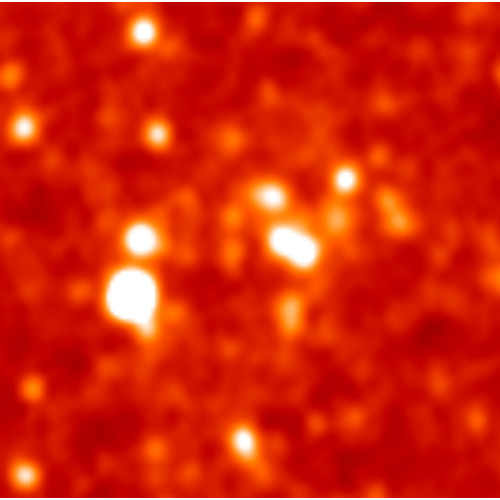
\includegraphics[width=\textwidth]{images/ARG000180p_ir.jpg}
                \caption{Infrared image.}
            \end{subfigure}
            \quad
            \begin{subfigure}{0.3\textwidth}
                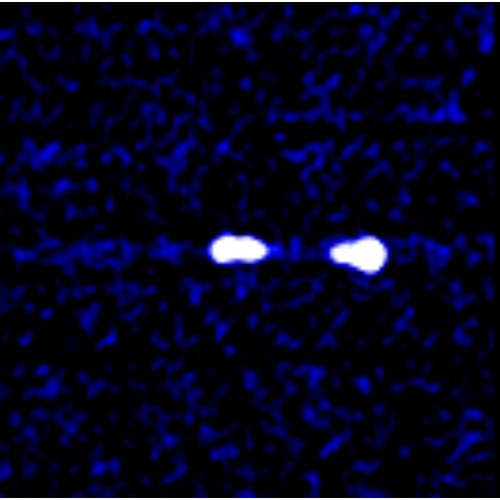
\includegraphics[width=\textwidth]{images/ARG000180p_radio.jpg}
                \caption{Radio image.}
            \end{subfigure}
            \caption{Infrared and radio images of Radio Galaxy Zoo subject ARG000180p.}
        \end{figure}

        Cross-identification is very difficult. Jets can be very complex, and it may not be clear where the radio source associated with the jets is located. For this reason, cross-identification is usually done by hand\cite{banfield15}, but this is impractical: There are already around $2.5 \times 10^6$ known radio sources, and future radio surveys such as the Evolutionary Map of the Universe (EMU)\cite{norris11} and WODAN\cite{röttgering11} are expected to find over $10^8$ new radio sources\cite{banfield15}. \emph{Radio Galaxy Zoo} is a crowdsourced citizen science project that tasks volunteers with cross-identifying 177461 images of radio sources through \href{http://radio.galaxyzoo.org}{a web interface}. [TODO(MatthewJA): details] To date\footnote{March 2016}, 94407 sources have been cross-identified, and Banfield et al.\cite{banfield15} report that when over 75\% of volunteers agree on a cross-identification, the volunteers are as good as expert astronomers at the cross-identification task.

        Of course, this still isn't enough to cross-identify all of the new radio sources we expect to find. The hope is that the cross-identifications provided by the Radio Galaxy Zoo volunteers can be used as labels for training a supervised machine learning algorithm on the cross-identification task. This hasn't been done before, and is the central task of my honours project.

    \section{Data Sources}

        In this section, I will describe the data files used in the project.

        Julie has provided me with four files:
        \begin{itemize}
            \item The ATLAS catalogue,
            \item CDFS radio and infrared images,
            \item ELAIS radio and infrared images, and
            \item Radio Galaxy Zoo subjects and classifications.
        \end{itemize}

        The ATLAS catalogue describes each object detected in ATLAS. However, the IDs of each object are actually different to the IDs in the images, so it's important to use the name as the primary ID of each object, and not the ID. More information is available in \href{https://github.com/chengsoonong/crowdastro/blob/master/docs/datasets/atlas.md}{the crowdastro documentation}.

        The CDFS and ELAIS data sets are formatted identically. Each subject in each set consists of an infrared PNG and FITS, a radio PNG and FITS, and an infrared PNG with the brightness contours of the radio PNG overlayed. There are both $2 \times 2$ and $5 \times 5$ patches provided around each subject. The FITS files contain metadata (mostly location data) for each image. Both datasets also include a metadata file that contians the spatial location of each subject.

        The Radio Galaxy Zoo subjects each correspond to a radio and infrared image. There are also a number of corresponding classifications; each of these represents one cross-identification by a volunteer of all radio sources in the image.

    \section{Potential Host Detection}

        Potential host detection is a subproblem of the cross-identification problem. If we have a list of potential host galaxies (hereafter \emph{potential hosts}), then we can classify each of these as $1$ if the potential host is the true host galaxy, and $0$ otherwise. This then turns the cross-identification problem into a binary classification task. The question, then, is: How do we detect potential hosts? I have found three possible methods.

        The first method is to find all local maxima in the infrared image of a subject, and then merge neighbouring local maxima. This requires preprocessing to reduce noise. The end result is still quite noisy and tends to pick up 200 -- 500 potential hosts per subject. This is explored in \href{https://github.com/chengsoonong/crowdastro/blob/master/notebooks/2_potential_host_counting.ipynb}{notebook 2}.

        The second method is to use a library such as scikit-image to detect blobs in the infrared image. This is more robust though it tends to merge galaxies that are very close together. This tends to find around 50 -- 80 potential hosts per subject. This is explored in \href{https://github.com/chengsoonong/crowdastro/blob/master/notebooks/10_potential_host_detection.ipynb}{notebook 10}.

        The third method is to consult the WISE object catalogues for the area covered by the subject, and use these objects. This will probably be a good method, since it will be in agreement with other astronomical results that use WISE data, but I haven't tried it yet.

    \section{Crowd Click Consensus --- Majority Vote}

        It is often the case that not every volunteer agrees on where the radio source is located for a given subject\footnote{It's also that case that not every volunteer agrees on which radio emissions are associated with the same source, but we're not sure how to deal with that right now, so I'm ignoring it.}. It's useful to know how often people disagree, and if they do disagree, how much. If it turns out that people don't disagree often, or they disagree a lot but there's always a clear majority, we can just pick the most common radio source location as the ``true'' location.

        This is explored in \href{https://github.com/chengsoonong/crowdastro/blob/master/notebooks/8_click_consensus_distribution.ipynb}{notebook 8}.

        TODO(MatthewJA): Write up results from notebook 8.

    \bibliographystyle{plain}
    \bibliography{papers}

\end{document}
